\newcommand\BOT{\operatorname{\text{\texttt{\$}}}} % begin of tape
\newcommand\EOT{\operatorname{\text{\texttt{!}}}} % begin of tape
%\newcommand\BLANK{\sqcup}

\sectionthree{Formal Definition of TM}
\begin{python0}
from solutions import *; clear()
\end{python0}

Here's the formal definition. Most of this won't be a surprise to
you by now. There's one thing I should mention. We will distinguish
between the alphabet of the string used to generate a language (the
$\Sigma$) and the alphabet that the TM can write on the tape.

\begin{defn}
A (deterministic) \textbf{Turing machine} TM $M$ is made up of
\begin{itemize}
 \item $Q$: a finite set of states.
 \item $\Sigma$: a finite set of input alphabet.
 \item $\Gamma$: a finite set of alphabet the TM using for read and write.
 $\Sigma$ is a subset of $\Gamma$.
 Furthermore the blank (or space) character $\sqcup$ is also in $\Gamma$.
 \item $q_0$: the initial state. This is in $Q$.
 \item $F$: the set of accepting states. $F$ is a subset of $Q$.
 \item $R$: the set of reject states. $R$ is a subset of $Q$.
 \item $B$: the blank symbol; this is in $\Gamma$ but not in $\Sigma$.
 In most TMs (and textbooks), this character is standardized and the same, 
 so it's usually not specified when describing a TM.
 \item $\delta : Q \times \Gamma \rightarrow Q 
\times \Gamma \times \{L, S, R\}$ is the transition function.
\end{itemize}
\end{defn}


Here's how you draw a TM given the above specification: Everything
is the same as a DFA. For the transitions, suppose you have
\[
 \delta(q, a) = (p, b, R)
\]
Then you draw a directed edge or transition from state $q$ to
state $p$ and label it $a/b, R$ or $a \rightarrow b, R$

To be formal about computation we will introduce the following
notation:

\begin{defn}
Let
\[
 x_1 \ldots x_m q x_{m+1} \ldots x_n
\]
to denote that fact that the TM current has it's read/write head
pointing to the $(m+1)$-st character on the tape $x_{m+1}$; this
will be the \textit{next} character the TM will read. This expression
\[
 x_1 \ldots x_m q x_{m+1} \ldots x_n
\]
is called
an \defone{instantaneous description} (ID). In some books this is
also called a \defone{configuration}. Of course if you're running
the TM with string $x$, the initial ID is
\[
q_0 x
\]
Of course these are all just notation for description a computation
of the TM. In particular if $\delta(q,a) = (b,p,R)$, then
\[
 x q a y \derive xb p y
\]
The read/write head over-writes $a$ with $b$ and moves right. Make
sure you understand that! If instead of that you have $\delta(q,a) =
(b,p,L)$, then
\[
 x c q a y \derive x p c b y
\]
so that the character being read, $a$, is over-written by $b$ and
the read/write head moves left. And if the transition if
$\delta(q,a) = (b,p,S)$, then the read/write head stays:
\[
 x q a y \derive x p b y
\]
As always, if we will use $\derive^*$ to note ``the same or at
least one derivation''.
\end{defn}

%-*-latex-*-

\begin{ex} 
  \label{ex:prob-00}
  \tinysidebar{\debug{exercises/{disc-prob-28/question.tex}}}

  \solutionlink{sol:prob-00}
  \qed
\end{ex} 
\begin{python0}
from solutions import *
add(label="ex:prob-00",
    srcfilename='exercises/discrete-probability/prob-00/answer.tex') 
\end{python0}


%-*-latex-*-

\begin{ex} 
  \label{ex:prob-00}
  \tinysidebar{\debug{exercises/{disc-prob-28/question.tex}}}

  \solutionlink{sol:prob-00}
  \qed
\end{ex} 
\begin{python0}
from solutions import *
add(label="ex:prob-00",
    srcfilename='exercises/discrete-probability/prob-00/answer.tex') 
\end{python0}

 
\begin{defn}
$x \in \Sigma^*$ is \defone{accepted} by $M$ is there is some $p
\in F$ such that
\[
 q_0 x \derive^* ypz
\]
for some strings $y,z$ in $\Gamma^*$. And, surprise-surprise, $L(M)$
is the set of strings accepted by $M$.
\end{defn}



There are many minor variations of the TM definition and they are
all essentially the same.
For instance:
\begin{tightlist}
\item Instead of having a set of accept states $F$, it's possible to redefine
the TM to have one single accept state without changing what the TM does.
In this case, the single accept state is usually written $q_\accept$.
\item Likewise it's possible to redefine a TM to have only one reject state.
In this case the special reject state is written $q_\reject$.
\item It's possible to rewrite the TM so that the read/write head does not
stay but always either move left or right.
In this case, the transition function is of the form:
\[
\delta : Q \times \Gamma \rightarrow Q 
\times \Gamma \times \{L, R\}
\]
\end{tightlist}

\begin{defn}
\begin{itemize}
 \item It's easy to show that in fact you only need one accepting
 state. (Why?) Therefore some books will just have a special state
 called $q_{\accept}$ for the only accepting state of the TM.
 \item Note that if the TM tries to move to the left while it's already at the leftmost
 position on the tape, then the machine crashes and stops running. The string is not accepted.
 Instead of allowing this to happen, some books will define a
 special state $q_{\reject}$. Whenever the TM enters the $q_\reject$ state it
 stops (or halt) and the string is not accepted.
 \item From the above, the TM can reject by either entering the
 state $q_{\reject}$ or by moving left on the leftmost position on
 the tape. It's easy to see that you really do not need both
 cases. You can rewrite the TM so that if it tries to fall off the
 left edge, you make the TM go into $q_{\reject}$ instead. Here's
 how you do it. Before running the TM, shift all the checks of the
 input string to the right by one, and insert a ``beginning of tape
 marker''; you can use any symbol not used for instance a common symbol in some books is `\$'.
 Then include a transition so that is the TM is reading
 the ``beginning of tape marker'' and it attempts to move the
 left, replace it with a transition that enters $q_{\reject}$
 instead. This will stop the machine before it falls off the left
 edge.
 \item Although according to the above definition of a TM there is
 a transition for every state $q$ and every symbol $a$ in
 $\Gamma$, it is customary not to include transitions that enters
 the state $q_{\reject}$. Therefore in some books some transitions
 are left out and the authors say that \lq\lq if the TM is in a state $q$
 and is reading a character $a$ but there is no applicable
 transition, the machine crashes and the string is rejected." This
 is just the same as including a transition from such a state and
 symbol to the rejecting state and of course you cannot exit the
 rejecting state.
 \end{itemize}
\end{defn}

\begin{defn}
A language is said to be
\defone{recognizable}
or
\defone{Turing recognizable} 
or
\defone{recursively enumerable} (r.e.)
if it is accepted by a TM.
\end{defn}

(Note: 
Computer Science is so new that many concepts still have multiple names.
Tune in after 100 hundred years to find out which name finally gets picked.)

Note one curious feature of the TM. It is possible for it to run
forever. That's not the case for either the DFA, NFA, or PDA. In
particular it's possible for the string not to accepted by the TM
entering the $q_{\reject}$ state, the TM crashes by moving to the
left while at the leftmost position on the tape, or it does not
enter an accepting state.

\begin{defn}
A language is said to be
\defone{decidable}
or
\defone{Turing decidable}
or
\defone{recursive} (rec)
if it is
accepted by a TM that always halts. A TM \defone{always halts} if
giving any input string, the TM will either reach an accepting
state or the rejecting state. The accepting state and rejecting
state are called \defone{halting states}.
\end{defn}


\newpage
\begin{eg}
It' easy to design a TM that accepts all strings with
characters from $\{a, b\}$:



\begin{center}
\begin{tikzpicture}[>=triangle 60,shorten >=0.5pt,node distance=2cm,auto,initial text=, double distance=2pt]
\node[state,initial,accepting] (A) at (  0,  0) {$q_0$};

\path[->]
(A) edge [loop above] node {$(a\rightarrow a, S), (b\rightarrow a, S),(\SPACE\rightarrow \SPACE, S), $} ()

;
\end{tikzpicture}
\end{center}
    


\end{eg}
  
\newpage
\begin{eg}
Let $L = \{a^n b^n c^n \,|\, n \geq 0\}$. We know that $L$ is not
a CFL. We will now prove that it is recursively enumerable, i.e.,
accepted by a TM.

TMs tend to large. So to simplify the specification of this TM,
transitions entering the $q_{\reject}$ state is not listed.

The idea is simple: Scan left and right, marking a single $a$ and
a single $b$ and a single $c$ in each right scan. We will need
special characters to denote that $a$,$b$ and $c$ are marked. We
will use $A$, $B$ and $C$ respectively. Of course if we cannot
find a $b$ or $c$ to match this $a$, the string is rejected. Now
once $c$ is marked, we move all the way to the left to look for
the first marked $a$ (i.e., $A$). Once that's found, we move
right. This would either be another $a$ or $B$. If it's $a$, we
repeat the process of marking $a$,$b$,$c$.

On the other hand if it's $B$, then there are no more $a$'s. Then
we just move right over all the marked characters (i.e., $B$ and
$C$) until we see a blank and accept the string. Of course if $b$
or $c$ is found, then the string is rejected; there shouldn't be
anymore $b$'s or $c$'s for the string to be accepted.

That's the main idea. Here's the TM. We will use $\BLANK$ to
denote the blank character.

\[
\begin{tabular}{|c|c|l|}
  \hline
  $(q,x)$ & $\delta(q,x)$ & \mbox{} \\
  \hline
  $(q_0,a)$ & $(q_1,A,R)$ & Start marking phase: Mark $a$ and move right \\
  $(q_1,a)$ & $(q_1,a,R)$ & Fast forward over $a$ \\
  $(q_1,B)$ & $(q_1,B,R)$ & Fast forward over $B$ \\
  $(q_1,b)$ & $(q_2,B,R)$ & Mark $b$ and move right \\
  $(q_2,b)$ & $(q_2,b,R)$ & Fast forward over $b$ \\
  $(q_2,C)$ & $(q_2,C,R)$ & Fast forward over $C$ \\
  $(q_2,c)$ & $(q_3,C,L)$ & Mark $c$ and move left \\
  $(q_3,C)$ & $(q_3,C,L)$ & Rewind over $C$ \\
  $(q_3,B)$ & $(q_3,B,L)$ & Rewind over $B$ \\
  $(q_3,b)$ & $(q_3,b,L)$ & Rewind over $b$ \\
  $(q_3,a)$ & $(q_3,a,L)$ & Rewind over $a$ \\
  $(q_3,A)$ & $(q_0,A,R)$ & On seeing $A$, go to state $q_0$\\
  $(q_0,B)$ & $(q_4,B,R)$ & Start scanning phase: read first $B$ and move right\\
  $(q_4,B)$ & $(q_4,B,R)$ & Fast forward over $B$ \\
  $(q_4,C)$ & $(q_5,C,R)$ & Read first C and move right\\
  $(q_5,C)$ & $(q_5,C,R)$ & Fast forward over $C$\\
  $(q_5,\SPACE)$ & $(q_{\accept},B,S)$ & Accept string when a $\BLANK$ is found\\
  \hline
\end{tabular}
\]

Make sure you draw the state (or transition) diagram. Again
transitions which are not labeled go to the $q_{\reject}$ state.
Instead of writing infinitely many blanks, we will write one blank
just beyond $abc$. If we need to we can add blanks when we need to
(actually, for this TM only one blank is needed.)

Now let's trace the execution of $M$ for the string $abc$.
\begin{align*}
q_0 abc\BLANK
 &\derive Aq_1bc \BLANK \\
 &\derive ABq_2c\BLANK \\
 &\derive Aq_3BC\BLANK \\
 &\derive q_3ABC\BLANK \\
 &\derive Aq_0BC\BLANK \\
 &\derive ABq_4C\BLANK \\
 &\derive ABCq_5\BLANK \\
 &\derive ABCq_{\accept}\BLANK \\
\end{align*}

Now try to trace the execution of the TM for $aabbcc$ and
$aabbccc$.
\end{eg}

[TODO: Check if \$ is better for begin-of-tape marker.
Might be easier for students to remember if \$ is used for
both begin-of-tape for TM and bottom of stakc for PDA.
Check if ! can be used for end of tape.

\newpage
\subsection{Single accept state}

In the formal definition of a TM, one can have any number of accept states.
In fact, you don't change the power of the machine if you assume that
there's exactly one accept state.
When there's one accept state, it's conventional to denote this
state as $q_\accept$.

%-*-latex-*-

\begin{ex} 
  \label{ex:prob-00}
  \tinysidebar{\debug{exercises/{disc-prob-28/question.tex}}}

  \solutionlink{sol:prob-00}
  \qed
\end{ex} 
\begin{python0}
from solutions import *
add(label="ex:prob-00",
    srcfilename='exercises/discrete-probability/prob-00/answer.tex') 
\end{python0}


\newpage
\subsection{Single reject state}

In the formal definition of a TM, one can have any number of reject states.
In fact, you don't change the power of the machine if you assume that
there's exactly one reject state.
When there's one accept state, it's conventional to denote this
state as $q_\accept$.

%-*-latex-*-

\begin{ex} 
  \label{ex:prob-00}
  \tinysidebar{\debug{exercises/{disc-prob-28/question.tex}}}

  \solutionlink{sol:prob-00}
  \qed
\end{ex} 
\begin{python0}
from solutions import *
add(label="ex:prob-00",
    srcfilename='exercises/discrete-probability/prob-00/answer.tex') 
\end{python0}


%-*-latex-*-

\begin{ex} 
  \label{ex:prob-00}
  \tinysidebar{\debug{exercises/{disc-prob-28/question.tex}}}

  \solutionlink{sol:prob-00}
  \qed
\end{ex} 
\begin{python0}
from solutions import *
add(label="ex:prob-00",
    srcfilename='exercises/discrete-probability/prob-00/answer.tex') 
\end{python0}

  
\newpage
\subsection{Read/write head that does not stay put}

In our definition of a TM, we allow a read/write head to move right, left,
or stay (put).
In Sipser's book, his definition does not allow the read/write head to
stay (put).
It seems that our TM has more power.
But in fact:

%-*-latex-*-

\begin{ex} 
  \label{ex:prob-00}
  \tinysidebar{\debug{exercises/{disc-prob-28/question.tex}}}

  \solutionlink{sol:prob-00}
  \qed
\end{ex} 
\begin{python0}
from solutions import *
add(label="ex:prob-00",
    srcfilename='exercises/discrete-probability/prob-00/answer.tex') 
\end{python0}


\newpage
\subsection{Moving off the left-end of the tape: begin-of-tape marker}

Note that our definition of a TM stipulates that when the read/write
head moves to the left on the first cell of the tape, i.e.,
it attempts beyond to move outside the tape (on the left),
the TM \lq\lq crashes'' meaning to say that
the TM halts and does not accept the input that it's running on.

In Sipser's book, he defines his TM so that
when a TM attempts to move left at the first cell, the read/write head
bounces back to the first cell and continues execution.

Let TM be our class of all TMs
and let $\TM'$ be the class of TMs from Sipser's book
in the sense that the read/write head will bounce back when it attempts
move to the left from the first cell.

%-*-latex-*-

\begin{ex} 
  \label{ex:prob-00}
  \tinysidebar{\debug{exercises/{disc-prob-28/question.tex}}}

  \solutionlink{sol:prob-00}
  \qed
\end{ex} 
\begin{python0}
from solutions import *
add(label="ex:prob-00",
    srcfilename='exercises/discrete-probability/prob-00/answer.tex') 
\end{python0}


\begin{eg} Here's a trick. To prevent the case where the TM moves
left while it's already at the leftmost position, you need to
shift all the character one position to the right.
Suppose the
symbol $\DOLLAR$ is not used. Suppose the TM is $M$. How would you
write a new TM that will shift the input by one space to the
right, put $\DOLLAR$ as the first character, and move the read/write
head so that it's about to read the first character of the input
string (i.e., first character to the right of $\DOLLAR$. Once this
pre-processing step is done, the new TM starts simulating the old
one. In other words in terms of ID, you want a TM $M'$ that will
do the following: Suppose the new start state is $q_0'$.
\[
 q_0x \derive \DOLLAR q_0x
\]
Since this modification can always be carried out on any TM, in
many books, it's assumed that the TM will never fall off the left
edge. In other words, these authors assume that it the TM tries to
move left on the leftmost spot, it will simply stay and not move.
\end{eg}


\newpage
\subsection{Output; transducer}

So far, we use a TM, $M$, to describe a language, i.e.,
given a string $x$, on running $M$ on $x$, we are interested if
$M$ accepts (i.e., $M$ enters an accept state)
or $M$ rejects (i.e., $M$ enters a reject state or runs without stopping).

We can also use a TM to produce an output string.
This is the string on the input tape when the TM halts.
(This means that an output makes sense only when the TM enters an accept
or a reject state, not when it runs on and on without stopping.)
In the case when the TM uses a begin-of-tape character, $\DOLLAR$,
then this $\DOLLAR$ is not part of the output.
If you use the end-of-tape character $\EOT$
to mark the end of output, $\EOT$ is not considered part of the output.
For instance if the TM halts with this on the input tape:

\begin{center}
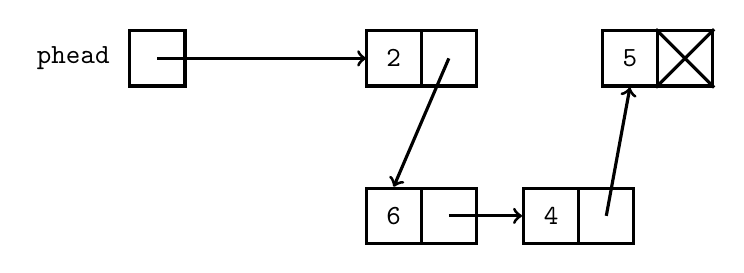
\begin{tikzpicture}

\draw (0.35, 0.35)
  node[draw, line width=0.04cm, , color=black,
       rounded corners=0cm, inner sep=0cm] {

\begin{minipage}[t][0.7cm]{0.7cm}
\mbox{}

\end{minipage}

};\draw (0.35, 0.35) node[color=black] {{\texttt{2}}};
\draw (1.0499999999999998, 0.35)
  node[draw, line width=0.04cm, , color=black,
       rounded corners=0cm, inner sep=0cm] {

\begin{minipage}[t][0.7cm]{0.7cm}
\mbox{}

\end{minipage}

};\draw (1.0499999999999998, 0.35) node[color=black] {{\texttt{}}};
\draw (0.35, -1.65)
  node[draw, line width=0.04cm, , color=black,
       rounded corners=0cm, inner sep=0cm] {

\begin{minipage}[t][0.7cm]{0.7cm}
\mbox{}

\end{minipage}

};\draw (0.35, -1.65) node[color=black] {{\texttt{6}}};
\draw (1.0499999999999998, -1.65)
  node[draw, line width=0.04cm, , color=black,
       rounded corners=0cm, inner sep=0cm] {

\begin{minipage}[t][0.7cm]{0.7cm}
\mbox{}

\end{minipage}

};\draw (1.0499999999999998, -1.65) node[color=black] {{\texttt{}}};
\draw (2.35, -1.65)
  node[draw, line width=0.04cm, , color=black,
       rounded corners=0cm, inner sep=0cm] {

\begin{minipage}[t][0.7cm]{0.7cm}
\mbox{}

\end{minipage}

};\draw (2.35, -1.65) node[color=black] {{\texttt{4}}};
\draw (3.0500000000000003, -1.65)
  node[draw, line width=0.04cm, , color=black,
       rounded corners=0cm, inner sep=0cm] {

\begin{minipage}[t][0.7cm]{0.7cm}
\mbox{}

\end{minipage}

};\draw (3.0500000000000003, -1.65) node[color=black] {{\texttt{}}};
\draw (3.35, 0.35)
  node[draw, line width=0.04cm, , color=black,
       rounded corners=0cm, inner sep=0cm] {

\begin{minipage}[t][0.7cm]{0.7cm}
\mbox{}

\end{minipage}

};\draw (3.35, 0.35) node[color=black] {{\texttt{5}}};
\draw (4.05, 0.35)
  node[draw, line width=0.04cm, , color=black,
       rounded corners=0cm, inner sep=0cm] {

\begin{minipage}[t][0.7cm]{0.7cm}
\mbox{}

\end{minipage}

};\draw (4.05, 0.35) node[color=black] {{\texttt{}}};\draw[line width=0.04cm,black,->] (1.05,0.35) to  (0.35,-1.28);
\draw[line width=0.04cm,black,->] (1.05,-1.65) to  (1.98,-1.65);
\draw[line width=0.04cm,black,->] (3.05,-1.65) to  (3.35,-0.02);
\draw[line width=0.04cm,black] (3.68,0.72) to  (4.42,-0.02);
\draw[line width=0.04cm,black] (4.42,0.72) to  (3.68,-0.02);

\draw (-2.65, 0.35)
  node[draw, line width=0.04cm, , color=black,
       rounded corners=0cm, inner sep=0cm] {

\begin{minipage}[t][0.7cm]{0.7cm}
\mbox{}

\end{minipage}

};\draw (-2.65, 0.35) node[color=black] {{\texttt{}}};\draw[line width=0.04cm,black,->] (-2.65,0.35) to  (0,0.35);

\draw (-3.7199999999999998, 0.35)
  node[draw, line width=0.04cm, , color=white,
       rounded corners=0cm, inner sep=0cm] {

\begin{minipage}[t][0.1cm]{0.1cm}
\mbox{}

\end{minipage}

};\draw (-3.7199999999999998, 0.35) node[color=black] {{\texttt{phead}}};
\end{tikzpicture}

\end{center}



then the ouptut is
\[
\text{\texttt{abaa}$\sqcup\sqcup$\texttt{a}$\sqcup$}
\]


Depending on the book you read,
sometimes the transducer will have a set of output characters which does not
include the space $\BLANK$.
In this case, the output will be all the characters up to but not including
the first space.
For instance

\begin{center}
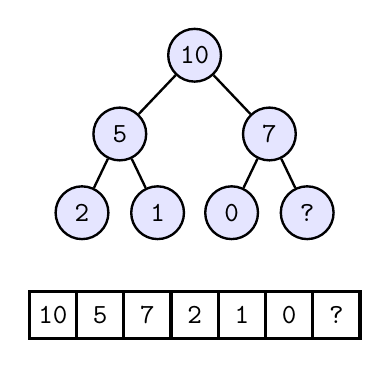
\begin{tikzpicture}

\fill[blue!10] (0.0, 0.0) circle (0.35);
\node [line width=0.03cm,black,minimum size=0.6699999999999999cm,draw,circle] at (0.0,0.0)(10){};\draw (0.0, 0.0) node[color=black] {\texttt{10}};
\fill[blue!10] (-0.95, -1.0) circle (0.35);
\node [line width=0.03cm,black,minimum size=0.6699999999999999cm,draw,circle] at (-0.95,-1.0)(5){};\draw (-0.95, -1.0) node[color=black] {\texttt{5}};
\fill[blue!10] (0.95, -1.0) circle (0.35);
\node [line width=0.03cm,black,minimum size=0.6699999999999999cm,draw,circle] at (0.95,-1.0)(7){};\draw (0.95, -1.0) node[color=black] {\texttt{7}};
\fill[blue!10] (-1.43, -2.0) circle (0.35);
\node [line width=0.03cm,black,minimum size=0.6699999999999999cm,draw,circle] at (-1.43,-2.0)(2){};\draw (-1.43, -2.0) node[color=black] {\texttt{2}};
\fill[blue!10] (-0.47, -2.0) circle (0.35);
\node [line width=0.03cm,black,minimum size=0.6699999999999999cm,draw,circle] at (-0.47,-2.0)(1){};\draw (-0.47, -2.0) node[color=black] {\texttt{1}};
\fill[blue!10] (0.47, -2.0) circle (0.35);
\node [line width=0.03cm,black,minimum size=0.6699999999999999cm,draw,circle] at (0.47,-2.0)(0){};\draw (0.47, -2.0) node[color=black] {\texttt{0}};
\fill[blue!10] (1.43, -2.0) circle (0.35);
\node [line width=0.03cm,black,minimum size=0.6699999999999999cm,draw,circle] at (1.43,-2.0)(?){};\draw (1.43, -2.0) node[color=black] {\texttt{?}};\draw[line width=0.03cm,black] (10) to  (5);
\draw[line width=0.03cm,black] (10) to  (7);
\draw[line width=0.03cm,black] (5) to  (2);
\draw[line width=0.03cm,black] (5) to  (1);
\draw[line width=0.03cm,black] (7) to  (0);
\draw[line width=0.03cm,black] (7) to  (?);

\draw (-1.8, -3.3)
  node[draw, line width=0.04cm, , color=black,
       rounded corners=0cm, inner sep=0cm] {

\begin{minipage}[t][0.6cm]{0.6cm}
\mbox{}

\end{minipage}

};\draw (-1.8, -3.3) node[color=black] {{\texttt{10}}};
\draw (-1.2, -3.3)
  node[draw, line width=0.04cm, , color=black,
       rounded corners=0cm, inner sep=0cm] {

\begin{minipage}[t][0.6cm]{0.6cm}
\mbox{}

\end{minipage}

};\draw (-1.2, -3.3) node[color=black] {{\texttt{5}}};
\draw (-0.6000000000000001, -3.3)
  node[draw, line width=0.04cm, , color=black,
       rounded corners=0cm, inner sep=0cm] {

\begin{minipage}[t][0.6cm]{0.6cm}
\mbox{}

\end{minipage}

};\draw (-0.6000000000000001, -3.3) node[color=black] {{\texttt{7}}};
\draw (-1.1102230246251565e-16, -3.3)
  node[draw, line width=0.04cm, , color=black,
       rounded corners=0cm, inner sep=0cm] {

\begin{minipage}[t][0.6cm]{0.6cm}
\mbox{}

\end{minipage}

};\draw (-1.1102230246251565e-16, -3.3) node[color=black] {{\texttt{2}}};
\draw (0.6, -3.3)
  node[draw, line width=0.04cm, , color=black,
       rounded corners=0cm, inner sep=0cm] {

\begin{minipage}[t][0.6cm]{0.6cm}
\mbox{}

\end{minipage}

};\draw (0.6, -3.3) node[color=black] {{\texttt{1}}};
\draw (1.2, -3.3)
  node[draw, line width=0.04cm, , color=black,
       rounded corners=0cm, inner sep=0cm] {

\begin{minipage}[t][0.6cm]{0.6cm}
\mbox{}

\end{minipage}

};\draw (1.2, -3.3) node[color=black] {{\texttt{0}}};
\draw (1.8, -3.3)
  node[draw, line width=0.04cm, , color=black,
       rounded corners=0cm, inner sep=0cm] {

\begin{minipage}[t][0.6cm]{0.6cm}
\mbox{}

\end{minipage}

};\draw (1.8, -3.3) node[color=black] {{\texttt{?}}};
\end{tikzpicture}

\end{center}



then the ouptut is
\[
\text{\texttt{abaa}}
\]

In fact, it's easy to modify the transducer so that once the output is written,
it shifts the non-space characters to the left by one, removing the
begin-of-tape character $\DOLLAR$
and it's also easy to replace the end-of-tape marker $\EOT$ by a space.
For instance in the input tape above, after shifting left by one and
replacing the $\EOT$ by a space,
we get

%-*-latex-*-

\begin{center}
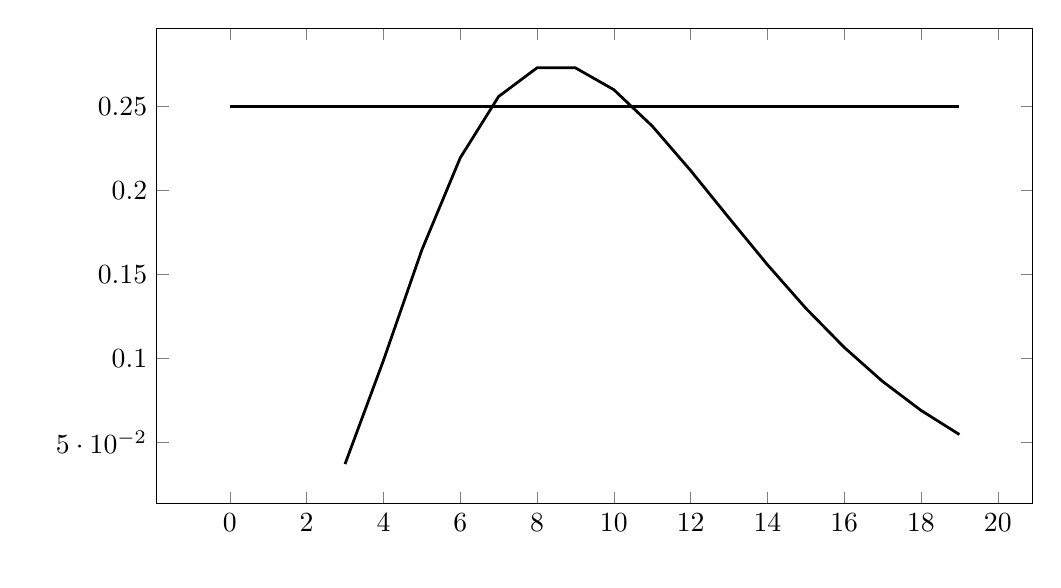
\begin{tikzpicture}[line width=1]
\begin{axis}[width=5in, height=3in,
             scatter/classes={a={mark=*,draw=black}},
             xlabel={\mbox{}},
             xlabel style={name=xlabel}, 
             ylabel={\mbox{}}, 
             legend style={
                at={(xlabel.south)},
                yshift=-1ex,
                anchor=north,
                legend cell align=left,
                },
        ]
]
\addplot[draw=black, line width=1] coordinates {(3, 0.03703703703703703)
(4, 0.0987654320987654)
(5, 0.16460905349794233)
(6, 0.21947873799725642)
(7, 0.2560585276634658)
(8, 0.2731290961743635)
(9, 0.2731290961743635)
(10, 0.26012294873748903)
(11, 0.23844603634269826)
(12, 0.2119520323046207)
(13, 0.18369176133067125)
(14, 0.15585967628056951)
(15, 0.12988306356714127)
(16, 0.10657071882432105)
(17, 0.08627153428635512)
(18, 0.06901722742908409)
(19, 0.05463863838135823)};\addplot[draw=black, line width=1] coordinates {(0, 0.25)
(1, 0.25)
(2, 0.25)
(3, 0.25)
(4, 0.25)
(5, 0.25)
(6, 0.25)
(7, 0.25)
(8, 0.25)
(9, 0.25)
(10, 0.25)
(11, 0.25)
(12, 0.25)
(13, 0.25)
(14, 0.25)
(15, 0.25)
(16, 0.25)
(17, 0.25)
(18, 0.25)
(19, 0.25)};
\end{axis}\end{tikzpicture}\end{center}


and then the transducer halts.
The output is then, again, the following:
\[
\text{\texttt{abaa}}
\]

When a TM is used for input/output, the TM is also called a
\defone{transducer}.
In the situation when a transducer does not halt, the output
is undefined.

It's common to have a symbol to denote the output function.
For instance, say $M$ is the transducer,
you can say \lq\lq Let $f_M$ be the output function of $M$.''
Suppose in the above, the input for $M$ was \texttt{ab}.
Then we write
\[
f_M(\text{\texttt{ab}}) = \text{\texttt{abaa}}
\]
as you would expect.
In terms of derivations of IDs, we have
\[
q_0 \text{\texttt{ab}} \derive^* f_M(\text{\texttt{ab}})q_\accept 
\]
assuming that when $M$ halts, the read/write head is about to read
the space after \texttt{abaa}.

By the way, for the case when you're using a TM as a transducer,
the important thing is the output and not whether the input was accepted or
not.
In other words, once the output is written on the input tape, you can
enter the accept state or the reject state -- it doesn't matter which one.
So for the case of a Turing transducer, some books will give such a
Turing machine a single halting state $q_{\text{halt}}$ that plays the role of
$q_\accept$ and $q_\reject$.

If a transducer $M$ always halts, then the output function is said to be
a \defone{total} function.
Otherwise (i.e., if $M$ can run forever so that  the output is undefined),
we say that output function is a \defone{partial} function.





\newpage
\subsection{Computation of $\N$}
  
\begin{eg}
You can use TM to compute numbers. For instance you can use the
string $111$ to represent $3$.
$0$ is represented by $\ep$.
Given this data format, you can
define the output of a TM $M$ by what's on the tape when then
machine halts. Can you define a TM that computes the twice
function. In other words $M(111)$ = $111111$, i.e., if you put
$111$ on the tape and run the machine, it should halt with
$111111$ on the tape.

The translation of a mathematical notation in our world
into one suitable as input to a TM is called an encoding.
So I would say that $11111$ is an encoding of $5$.
It's common to use $\langle x \rangle$ to denote an encoding of
$x$.
So I would write for instance $\langle 5 \rangle = 11111$.

If the TM does not halt on input $x$, then
we say $M(x)$ \defone{diverges}.
[PUT THIS SOMEWHERE ELSE.]

\begin{itemize}
 \item You can design a
 TM to add numbers. For instance to add two 3 and 5, the input to
 the TM is $111011111$, i.e., $1^301^5$.
 The expected output is $11111111$, i.e., $1^8$.
 Can
 you design such a TM?
 In general, can you design a Turing machine (a transducer)
 $M$ such that if $f_M$
 is the output function of $M$, then
 \[
 f_M(1^m 0 1^n) = 1^{m+n}
 \]
\item Can you design one to perform subtract
 of the form $m-n$ where $m\geq n$? In other words you want to
 design a TM $M$ such that if $g_M$ is the output function,
 then $g_M(1^m 0 1^n) = 1^{m-n}$.
 \item Can you design a TM to do multiplication? For instance to
 compute the product of 3 and 4, you run the machine with
 $11101111$ and get $111111111111$.
 \item Can you design a TM $M$ that can computer powers of 2? For instance
 $M(1) = 11$, $M(111) = 11111111$.
\end{itemize}
\end{eg}

You can of course combine all the above features into a single
TM.
For instance you can use $1$ to denote $+$, $11$ to denote $-$, and
$111$ to denote $*$.
In that case to compute $10 + 15$, you use the input
$1^{10}0101^{15}$;
to compute $10 - 5$, you use $1^{10}01101^{5}$;
to compute $10 * 15$, you use $1^{10}011101^{15}$.

%-*-latex-*-

\begin{ex} 
  \label{ex:prob-00}
  \tinysidebar{\debug{exercises/{disc-prob-28/question.tex}}}

  \solutionlink{sol:prob-00}
  \qed
\end{ex} 
\begin{python0}
from solutions import *
add(label="ex:prob-00",
    srcfilename='exercises/discrete-probability/prob-00/answer.tex') 
\end{python0}


%-*-latex-*-

\begin{ex} 
  \label{ex:prob-00}
  \tinysidebar{\debug{exercises/{disc-prob-28/question.tex}}}

  \solutionlink{sol:prob-00}
  \qed
\end{ex} 
\begin{python0}
from solutions import *
add(label="ex:prob-00",
    srcfilename='exercises/discrete-probability/prob-00/answer.tex') 
\end{python0}


%-*-latex-*-

\begin{ex} 
  \label{ex:prob-00}
  \tinysidebar{\debug{exercises/{disc-prob-28/question.tex}}}

  \solutionlink{sol:prob-00}
  \qed
\end{ex} 
\begin{python0}
from solutions import *
add(label="ex:prob-00",
    srcfilename='exercises/discrete-probability/prob-00/answer.tex') 
\end{python0}


%-*-latex-*-

\begin{ex} 
  \label{ex:prob-00}
  \tinysidebar{\debug{exercises/{disc-prob-28/question.tex}}}

  \solutionlink{sol:prob-00}
  \qed
\end{ex} 
\begin{python0}
from solutions import *
add(label="ex:prob-00",
    srcfilename='exercises/discrete-probability/prob-00/answer.tex') 
\end{python0}


%-*-latex-*-

\begin{ex} 
  \label{ex:prob-00}
  \tinysidebar{\debug{exercises/{disc-prob-28/question.tex}}}

  \solutionlink{sol:prob-00}
  \qed
\end{ex} 
\begin{python0}
from solutions import *
add(label="ex:prob-00",
    srcfilename='exercises/discrete-probability/prob-00/answer.tex') 
\end{python0}


\begin{eg}
Design a TM that accepts $\{a^nb^nc^n \,|\, n \equiv 1
\,\,\,(\operatorname{mod} \, 4)\}$. The solution is easy. First
the TM checks the input is of the form $a^nb^nc^n$. (We've already
done that). After this point if the $a$'s might be marked with
another character. Let's say it's been replaced by $A$'s. First
the TM go to the leftmost $A$. It moves right so that the
read/write head is reading the next $A$ (or possibly $B$). It will
then continually read 4 $A$'s until a $B$ is reached. If that can
be done, then TM enters the $q_{\accept}$ state. Otherwise it
enters the $q_{\reject}$ state.
\end{eg}


There are many other computational models ($\lambda$--calculus
random access machines, general recursive functions, etc.) But in
the end they are all proven to be only as powerful as the original
Turing machines. Therefore solving a problem algorithmically is
believed to be equivalent to solving a problem using a Turing
machine. This is known as the
\defone{Church-Turing thesis}.



\newpage
\subsection{Beginning-of-tape}

It's convenient to have a special character to mark the beginning of
the input tape.
This is useful for instance if you want to \lq\lq rewind'' the read-write
head to the beginning before processing the input tape from left-to-right.
I will use $\DOLLAR$ to denote the beginning-of-tape character.
This is a character in $\Gamma$ but not in $\Sigma$.

In the Sipser book, he has the assumption that \lq\lq when the read-write
head attempts to move left at the first square of the input tape,
then it does not move."

With the beginning-of-tape character $\DOLLAR$ at the beginning of the
input tape just before the input, we can simulate the behavior of
Sipser's TM by adding this transition:
\[
\delta(q, \DOLLAR) = (q, \DOLLAR, R)
\]
for all $q \in Q$.

%-*-latex-*-

\begin{ex} 
  \label{ex:prob-00}
  \tinysidebar{\debug{exercises/{disc-prob-28/question.tex}}}

  \solutionlink{sol:prob-00}
  \qed
\end{ex} 
\begin{python0}
from solutions import *
add(label="ex:prob-00",
    srcfilename='exercises/discrete-probability/prob-00/answer.tex') 
\end{python0}


\newpage
\subsection{End-of-tape}

Besides having the beginning-of-tape marker $\BOT$,
we can also have an end-of-tape marker $\EOT$.
(This is my name.)
The end-of-tape marker is meant to mark where the read-write head has reached.
It does not mean that the tape is finite.
For instance, say you have the following input tape (with beginning-of
tape marker):

\begin{center}
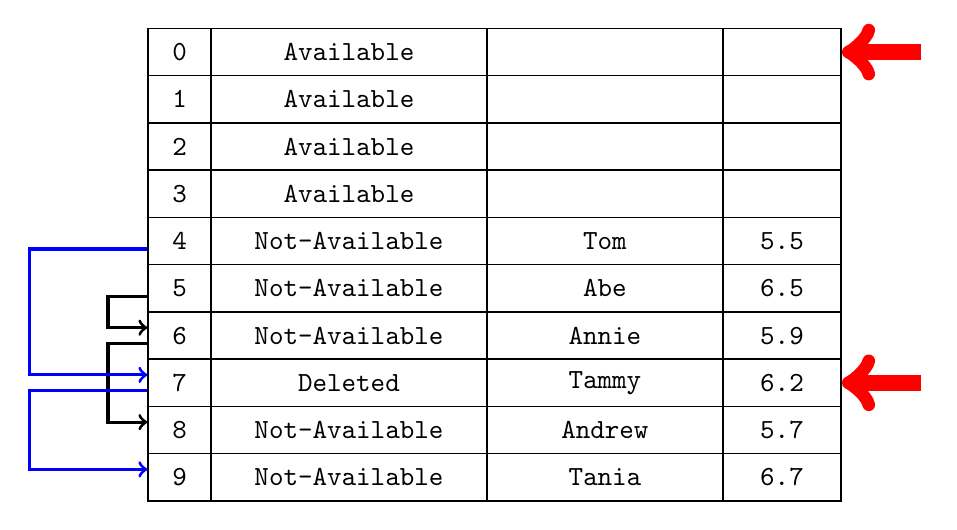
\begin{tikzpicture}

\draw (1.4, 0.7)
  node[draw, line width=0.02cm, , color=black,
       rounded corners=0cm, inner sep=0cm] {

\begin{minipage}[t][0.6cm]{0.8cm}
\mbox{}

\end{minipage}

};\draw (1.4, 0.7) node[color=black] {{\texttt{0}}};
\draw (3.55, 0.7)
  node[draw, line width=0.02cm, , color=black,
       rounded corners=0cm, inner sep=0cm] {

\begin{minipage}[t][0.6cm]{3.5cm}
\mbox{}

\end{minipage}

};\draw (3.55, 0.7) node[color=black] {{\texttt{Available}}};
\draw (6.800000000000001, 0.7)
  node[draw, line width=0.02cm, , color=black,
       rounded corners=0cm, inner sep=0cm] {

\begin{minipage}[t][0.6cm]{3.0cm}
\mbox{}

\end{minipage}

};\draw (6.800000000000001, 0.7) node[color=black] {{\texttt{}}};
\draw (9.05, 0.7)
  node[draw, line width=0.02cm, , color=black,
       rounded corners=0cm, inner sep=0cm] {

\begin{minipage}[t][0.6cm]{1.5cm}
\mbox{}

\end{minipage}

};\draw (9.05, 0.7) node[color=black] {{\texttt{}}};
\draw (1.4, 0.09999999999999987)
  node[draw, line width=0.02cm, , color=black,
       rounded corners=0cm, inner sep=0cm] {

\begin{minipage}[t][0.6cm]{0.8cm}
\mbox{}

\end{minipage}

};\draw (1.4, 0.09999999999999987) node[color=black] {{\texttt{1}}};
\draw (3.55, 0.09999999999999987)
  node[draw, line width=0.02cm, , color=black,
       rounded corners=0cm, inner sep=0cm] {

\begin{minipage}[t][0.6cm]{3.5cm}
\mbox{}

\end{minipage}

};\draw (3.55, 0.09999999999999987) node[color=black] {{\texttt{Available}}};
\draw (6.800000000000001, 0.09999999999999987)
  node[draw, line width=0.02cm, , color=black,
       rounded corners=0cm, inner sep=0cm] {

\begin{minipage}[t][0.6cm]{3.0cm}
\mbox{}

\end{minipage}

};\draw (6.800000000000001, 0.09999999999999987) node[color=black] {{\texttt{}}};
\draw (9.05, 0.09999999999999987)
  node[draw, line width=0.02cm, , color=black,
       rounded corners=0cm, inner sep=0cm] {

\begin{minipage}[t][0.6cm]{1.5cm}
\mbox{}

\end{minipage}

};\draw (9.05, 0.09999999999999987) node[color=black] {{\texttt{}}};
\draw (1.4, -0.5000000000000002)
  node[draw, line width=0.02cm, , color=black,
       rounded corners=0cm, inner sep=0cm] {

\begin{minipage}[t][0.6cm]{0.8cm}
\mbox{}

\end{minipage}

};\draw (1.4, -0.5000000000000002) node[color=black] {{\texttt{2}}};
\draw (3.55, -0.5000000000000002)
  node[draw, line width=0.02cm, , color=black,
       rounded corners=0cm, inner sep=0cm] {

\begin{minipage}[t][0.6cm]{3.5cm}
\mbox{}

\end{minipage}

};\draw (3.55, -0.5000000000000002) node[color=black] {{\texttt{Available}}};
\draw (6.800000000000001, -0.5000000000000002)
  node[draw, line width=0.02cm, , color=black,
       rounded corners=0cm, inner sep=0cm] {

\begin{minipage}[t][0.6cm]{3.0cm}
\mbox{}

\end{minipage}

};\draw (6.800000000000001, -0.5000000000000002) node[color=black] {{\texttt{}}};
\draw (9.05, -0.5000000000000002)
  node[draw, line width=0.02cm, , color=black,
       rounded corners=0cm, inner sep=0cm] {

\begin{minipage}[t][0.6cm]{1.5cm}
\mbox{}

\end{minipage}

};\draw (9.05, -0.5000000000000002) node[color=black] {{\texttt{}}};
\draw (1.4, -1.1000000000000003)
  node[draw, line width=0.02cm, , color=black,
       rounded corners=0cm, inner sep=0cm] {

\begin{minipage}[t][0.6cm]{0.8cm}
\mbox{}

\end{minipage}

};\draw (1.4, -1.1000000000000003) node[color=black] {{\texttt{3}}};
\draw (3.55, -1.1000000000000003)
  node[draw, line width=0.02cm, , color=black,
       rounded corners=0cm, inner sep=0cm] {

\begin{minipage}[t][0.6cm]{3.5cm}
\mbox{}

\end{minipage}

};\draw (3.55, -1.1000000000000003) node[color=black] {{\texttt{Available}}};
\draw (6.800000000000001, -1.1000000000000003)
  node[draw, line width=0.02cm, , color=black,
       rounded corners=0cm, inner sep=0cm] {

\begin{minipage}[t][0.6cm]{3.0cm}
\mbox{}

\end{minipage}

};\draw (6.800000000000001, -1.1000000000000003) node[color=black] {{\texttt{}}};
\draw (9.05, -1.1000000000000003)
  node[draw, line width=0.02cm, , color=black,
       rounded corners=0cm, inner sep=0cm] {

\begin{minipage}[t][0.6cm]{1.5cm}
\mbox{}

\end{minipage}

};\draw (9.05, -1.1000000000000003) node[color=black] {{\texttt{}}};
\draw (1.4, -1.7000000000000002)
  node[draw, line width=0.02cm, , color=black,
       rounded corners=0cm, inner sep=0cm] {

\begin{minipage}[t][0.6cm]{0.8cm}
\mbox{}

\end{minipage}

};\draw (1.4, -1.7000000000000002) node[color=black] {{\texttt{4}}};
\draw (3.55, -1.7000000000000002)
  node[draw, line width=0.02cm, , color=black,
       rounded corners=0cm, inner sep=0cm] {

\begin{minipage}[t][0.6cm]{3.5cm}
\mbox{}

\end{minipage}

};\draw (3.55, -1.7000000000000002) node[color=black] {{\texttt{Not-Available}}};
\draw (6.800000000000001, -1.7000000000000002)
  node[draw, line width=0.02cm, , color=black,
       rounded corners=0cm, inner sep=0cm] {

\begin{minipage}[t][0.6cm]{3.0cm}
\mbox{}

\end{minipage}

};\draw (6.800000000000001, -1.7000000000000002) node[color=black] {{\texttt{Tom}}};
\draw (9.05, -1.7000000000000002)
  node[draw, line width=0.02cm, , color=black,
       rounded corners=0cm, inner sep=0cm] {

\begin{minipage}[t][0.6cm]{1.5cm}
\mbox{}

\end{minipage}

};\draw (9.05, -1.7000000000000002) node[color=black] {{\texttt{5.5}}};
\draw (1.4, -2.3000000000000003)
  node[draw, line width=0.02cm, , color=black,
       rounded corners=0cm, inner sep=0cm] {

\begin{minipage}[t][0.6cm]{0.8cm}
\mbox{}

\end{minipage}

};\draw (1.4, -2.3000000000000003) node[color=black] {{\texttt{5}}};
\draw (3.55, -2.3000000000000003)
  node[draw, line width=0.02cm, , color=black,
       rounded corners=0cm, inner sep=0cm] {

\begin{minipage}[t][0.6cm]{3.5cm}
\mbox{}

\end{minipage}

};\draw (3.55, -2.3000000000000003) node[color=black] {{\texttt{Not-Available}}};
\draw (6.800000000000001, -2.3000000000000003)
  node[draw, line width=0.02cm, , color=black,
       rounded corners=0cm, inner sep=0cm] {

\begin{minipage}[t][0.6cm]{3.0cm}
\mbox{}

\end{minipage}

};\draw (6.800000000000001, -2.3000000000000003) node[color=black] {{\texttt{Abe}}};
\draw (9.05, -2.3000000000000003)
  node[draw, line width=0.02cm, , color=black,
       rounded corners=0cm, inner sep=0cm] {

\begin{minipage}[t][0.6cm]{1.5cm}
\mbox{}

\end{minipage}

};\draw (9.05, -2.3000000000000003) node[color=black] {{\texttt{6.5}}};
\draw (1.4, -2.9000000000000004)
  node[draw, line width=0.02cm, , color=black,
       rounded corners=0cm, inner sep=0cm] {

\begin{minipage}[t][0.6cm]{0.8cm}
\mbox{}

\end{minipage}

};\draw (1.4, -2.9000000000000004) node[color=black] {{\texttt{6}}};
\draw (3.55, -2.9000000000000004)
  node[draw, line width=0.02cm, , color=black,
       rounded corners=0cm, inner sep=0cm] {

\begin{minipage}[t][0.6cm]{3.5cm}
\mbox{}

\end{minipage}

};\draw (3.55, -2.9000000000000004) node[color=black] {{\texttt{Not-Available}}};
\draw (6.800000000000001, -2.9000000000000004)
  node[draw, line width=0.02cm, , color=black,
       rounded corners=0cm, inner sep=0cm] {

\begin{minipage}[t][0.6cm]{3.0cm}
\mbox{}

\end{minipage}

};\draw (6.800000000000001, -2.9000000000000004) node[color=black] {{\texttt{Annie}}};
\draw (9.05, -2.9000000000000004)
  node[draw, line width=0.02cm, , color=black,
       rounded corners=0cm, inner sep=0cm] {

\begin{minipage}[t][0.6cm]{1.5cm}
\mbox{}

\end{minipage}

};\draw (9.05, -2.9000000000000004) node[color=black] {{\texttt{5.9}}};
\draw (1.4, -3.500000000000001)
  node[draw, line width=0.02cm, , color=black,
       rounded corners=0cm, inner sep=0cm] {

\begin{minipage}[t][0.6cm]{0.8cm}
\mbox{}

\end{minipage}

};\draw (1.4, -3.500000000000001) node[color=black] {{\texttt{7}}};
\draw (3.55, -3.500000000000001)
  node[draw, line width=0.02cm, , color=black,
       rounded corners=0cm, inner sep=0cm] {

\begin{minipage}[t][0.6cm]{3.5cm}
\mbox{}

\end{minipage}

};\draw (3.55, -3.500000000000001) node[color=black] {{\texttt{Deleted}}};
\draw (6.800000000000001, -3.500000000000001)
  node[draw, line width=0.02cm, , color=black,
       rounded corners=0cm, inner sep=0cm] {

\begin{minipage}[t][0.6cm]{3.0cm}
\mbox{}

\end{minipage}

};\draw (6.800000000000001, -3.500000000000001) node[color=black] {{\texttt{Tammy}}};
\draw (9.05, -3.500000000000001)
  node[draw, line width=0.02cm, , color=black,
       rounded corners=0cm, inner sep=0cm] {

\begin{minipage}[t][0.6cm]{1.5cm}
\mbox{}

\end{minipage}

};\draw (9.05, -3.500000000000001) node[color=black] {{\texttt{6.2}}};
\draw (1.4, -4.1000000000000005)
  node[draw, line width=0.02cm, , color=black,
       rounded corners=0cm, inner sep=0cm] {

\begin{minipage}[t][0.6cm]{0.8cm}
\mbox{}

\end{minipage}

};\draw (1.4, -4.1000000000000005) node[color=black] {{\texttt{8}}};
\draw (3.55, -4.1000000000000005)
  node[draw, line width=0.02cm, , color=black,
       rounded corners=0cm, inner sep=0cm] {

\begin{minipage}[t][0.6cm]{3.5cm}
\mbox{}

\end{minipage}

};\draw (3.55, -4.1000000000000005) node[color=black] {{\texttt{Not-Available}}};
\draw (6.800000000000001, -4.1000000000000005)
  node[draw, line width=0.02cm, , color=black,
       rounded corners=0cm, inner sep=0cm] {

\begin{minipage}[t][0.6cm]{3.0cm}
\mbox{}

\end{minipage}

};\draw (6.800000000000001, -4.1000000000000005) node[color=black] {{\texttt{Andrew}}};
\draw (9.05, -4.1000000000000005)
  node[draw, line width=0.02cm, , color=black,
       rounded corners=0cm, inner sep=0cm] {

\begin{minipage}[t][0.6cm]{1.5cm}
\mbox{}

\end{minipage}

};\draw (9.05, -4.1000000000000005) node[color=black] {{\texttt{5.7}}};
\draw (1.4, -4.7)
  node[draw, line width=0.02cm, , color=black,
       rounded corners=0cm, inner sep=0cm] {

\begin{minipage}[t][0.6cm]{0.8cm}
\mbox{}

\end{minipage}

};\draw (1.4, -4.7) node[color=black] {{\texttt{9}}};
\draw (3.55, -4.7)
  node[draw, line width=0.02cm, , color=black,
       rounded corners=0cm, inner sep=0cm] {

\begin{minipage}[t][0.6cm]{3.5cm}
\mbox{}

\end{minipage}

};\draw (3.55, -4.7) node[color=black] {{\texttt{Not-Available}}};
\draw (6.800000000000001, -4.7)
  node[draw, line width=0.02cm, , color=black,
       rounded corners=0cm, inner sep=0cm] {

\begin{minipage}[t][0.6cm]{3.0cm}
\mbox{}

\end{minipage}

};\draw (6.800000000000001, -4.7) node[color=black] {{\texttt{Tania}}};
\draw (9.05, -4.7)
  node[draw, line width=0.02cm, , color=black,
       rounded corners=0cm, inner sep=0cm] {

\begin{minipage}[t][0.6cm]{1.5cm}
\mbox{}

\end{minipage}

};\draw (9.05, -4.7) node[color=black] {{\texttt{6.7}}};\draw[line width=0.04cm,black,->] (0.99,-2.4) to  (0.49,-2.4) to  (0.49,-2.8) to  (0.99,-2.8);
\draw[line width=0.04cm,black,->] (0.99,-3.0) to  (0.49,-3.0) to  (0.49,-4.0) to  (0.99,-4.0);
\draw[line width=0.04cm,blue,->] (0.99,-1.8) to  (-0.51,-1.8) to  (-0.51,-3.4) to  (0.99,-3.4);
\draw[line width=0.04cm,blue,->] (0.99,-3.6) to  (-0.51,-3.6) to  (-0.51,-4.6) to  (0.99,-4.6);
\draw[line width=0.2cm,red,->] (10.81,-3.5) to  (9.81,-3.5);
\draw[line width=0.2cm,red,->] (10.81,0.7) to  (9.81,0.7);
\end{tikzpicture}

\end{center}



and the read-write head actually reached the space after
the \texttt{a} furthest from the $\BOT$, then
this is what the input tape looks like when it has an end-of-tape marker:

\begin{center}
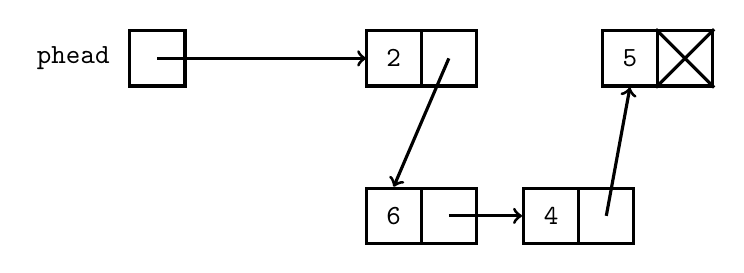
\begin{tikzpicture}

\draw (0.35, 0.35)
  node[draw, line width=0.04cm, , color=black,
       rounded corners=0cm, inner sep=0cm] {

\begin{minipage}[t][0.7cm]{0.7cm}
\mbox{}

\end{minipage}

};\draw (0.35, 0.35) node[color=black] {{\texttt{2}}};
\draw (1.0499999999999998, 0.35)
  node[draw, line width=0.04cm, , color=black,
       rounded corners=0cm, inner sep=0cm] {

\begin{minipage}[t][0.7cm]{0.7cm}
\mbox{}

\end{minipage}

};\draw (1.0499999999999998, 0.35) node[color=black] {{\texttt{}}};
\draw (0.35, -1.65)
  node[draw, line width=0.04cm, , color=black,
       rounded corners=0cm, inner sep=0cm] {

\begin{minipage}[t][0.7cm]{0.7cm}
\mbox{}

\end{minipage}

};\draw (0.35, -1.65) node[color=black] {{\texttt{6}}};
\draw (1.0499999999999998, -1.65)
  node[draw, line width=0.04cm, , color=black,
       rounded corners=0cm, inner sep=0cm] {

\begin{minipage}[t][0.7cm]{0.7cm}
\mbox{}

\end{minipage}

};\draw (1.0499999999999998, -1.65) node[color=black] {{\texttt{}}};
\draw (2.35, -1.65)
  node[draw, line width=0.04cm, , color=black,
       rounded corners=0cm, inner sep=0cm] {

\begin{minipage}[t][0.7cm]{0.7cm}
\mbox{}

\end{minipage}

};\draw (2.35, -1.65) node[color=black] {{\texttt{4}}};
\draw (3.0500000000000003, -1.65)
  node[draw, line width=0.04cm, , color=black,
       rounded corners=0cm, inner sep=0cm] {

\begin{minipage}[t][0.7cm]{0.7cm}
\mbox{}

\end{minipage}

};\draw (3.0500000000000003, -1.65) node[color=black] {{\texttt{}}};
\draw (3.35, 0.35)
  node[draw, line width=0.04cm, , color=black,
       rounded corners=0cm, inner sep=0cm] {

\begin{minipage}[t][0.7cm]{0.7cm}
\mbox{}

\end{minipage}

};\draw (3.35, 0.35) node[color=black] {{\texttt{5}}};
\draw (4.05, 0.35)
  node[draw, line width=0.04cm, , color=black,
       rounded corners=0cm, inner sep=0cm] {

\begin{minipage}[t][0.7cm]{0.7cm}
\mbox{}

\end{minipage}

};\draw (4.05, 0.35) node[color=black] {{\texttt{}}};\draw[line width=0.04cm,black,->] (1.05,0.35) to  (0.35,-1.28);
\draw[line width=0.04cm,black,->] (1.05,-1.65) to  (1.98,-1.65);
\draw[line width=0.04cm,black,->] (3.05,-1.65) to  (3.35,-0.02);
\draw[line width=0.04cm,black] (3.68,0.72) to  (4.42,-0.02);
\draw[line width=0.04cm,black] (4.42,0.72) to  (3.68,-0.02);

\draw (-2.65, 0.35)
  node[draw, line width=0.04cm, , color=black,
       rounded corners=0cm, inner sep=0cm] {

\begin{minipage}[t][0.7cm]{0.7cm}
\mbox{}

\end{minipage}

};\draw (-2.65, 0.35) node[color=black] {{\texttt{}}};\draw[line width=0.04cm,black,->] (-2.65,0.35) to  (0,0.35);

\draw (-3.7199999999999998, 0.35)
  node[draw, line width=0.04cm, , color=white,
       rounded corners=0cm, inner sep=0cm] {

\begin{minipage}[t][0.1cm]{0.1cm}
\mbox{}

\end{minipage}

};\draw (-3.7199999999999998, 0.35) node[color=black] {{\texttt{phead}}};
\end{tikzpicture}

\end{center}



The end-of-tape marker is useful if I want to move the chunk of 
characters that is processed so far to the right by say one square.

%-*-latex-*-

\begin{ex} 
  \label{ex:prob-00}
  \tinysidebar{\debug{exercises/{disc-prob-28/question.tex}}}

  \solutionlink{sol:prob-00}
  \qed
\end{ex} 
\begin{python0}
from solutions import *
add(label="ex:prob-00",
    srcfilename='exercises/discrete-probability/prob-00/answer.tex') 
\end{python0}


%-*-latex-*-

\begin{ex} 
  \label{ex:prob-00}
  \tinysidebar{\debug{exercises/{disc-prob-28/question.tex}}}

  \solutionlink{sol:prob-00}
  \qed
\end{ex} 
\begin{python0}
from solutions import *
add(label="ex:prob-00",
    srcfilename='exercises/discrete-probability/prob-00/answer.tex') 
\end{python0}

